\subsection{MongoDB}
Für die Abbildung des Anwendungsszenarios wurde sich dafür entschieden die Datensätze, bis auf kleine Korrekturen, unverändert zu übernehmen. Dafür wurde jeder Datensatz, jede Zeile der CSV-Datei, als ein Dokument importiert. Um schnelle Abfragen auf die Daten zu ermöglichen wurden häufig genutzte Attribute indiziert.

\subsubsection{Import der Daten}
Die Beschreibung des Datenimports ist mit Hilfe des ETL-Prozesses strukturiert:

\emph{Extraktion} -
Da die Daten in Form einer CSV-Datei bereit gestellt wurden, entfällt dieser Schritt. Allerdings müssen zwei kleine Anpassungen an der CSV-Datei vorgenommen werden:

\begin{itemize}
\item \textit{Umlaute korrigieren} - Die Umlaute in der CSV-Datei wurden, vermutlich durch den Export aus dem Quellsystem, fehlerhaft dargestellt. Diese wurde so ersetzt, dass sie wieder menschenlesbar sind.
\item \textit{Kopfzeile anpassen} - Die Werte in der Kopfzeile listen die Attributnamen auf. Diese werden später die Schlüssel der Werte des Dokuments in der Datenbank sein. Schlüsselnamen dürfen weder Leerzeichen noch Umlaute enthalten. Somit wurden die Leerzeichen entfernt und durch Unterstriche ,,\_`` ersetzt sowie alle Umlaute mit einfachen Vokalen dargestellt. So wurde beispielsweise aus ,,\"a`` ae oder aus ,,\ss{}`` ss.
\end{itemize}

\emph{Transformation} -
Da MongoDB Imports primär über JSON erwartet, musste die CSV-Datei in das JSON-Format transformiert werden. Die Transformation der Daten wurde mit Hilfe eines Online Tools durchgeführt. Diese ist unter der URL \url{http://www.csvjson.com/csv2json} \citep{drapeau01} zu finden.

\emph{Laden} -
Der Import in die MongoDB erfolgt über die MongoDB-Konsole. Um die Arbeit hier etwas zu vereinfachen wurde das GUI-Tool ,,RoboMongo`` verwendet. Die Syntax des Import-Befehls ist Listing \ref{lst:mongodb_import} zu entnehmen. Dabei können mehrere Dokumente in einem Array per Komma getrennt gleichzeitig importiert werden. \\

%https://en.wikibooks.org/wiki/LaTeX/Source_Code_Listings
\begin{lstlisting}[caption={MongoDB Importfunktion},language=java,captionpos=t,numbers=none, numberstyle=\tiny,basicstyle=\scriptsize,breaklines=true]
db.getCollection('Collection_Name').insert([{Document01},{Document02},
	{"Attribut01":"Wert01", "Attribut02":"Wert02"}])
\end{lstlisting}\label{lst:mongodb_import}

Allerdings sind die 1639 Datensätze mit 32,7 MB Gesamtgröße zu groß für einen Import. Das Maximum hier liegt bei circa 16 MB. Also wurden die Datensätze in drei Teile aufgeteilt und nacheinander importiert.

\subsubsection{Anwendungsszenario}
Die erstellte Website soll von Professoren und Studenten dafür genutzt werden, um nach Informationen über alle bisherigen Abschlussarbeiten suchen zu können. Dies kann beispielsweise für Professoren statistische oder Auswertungszwecke verfolgen oder für Studenten, welche auf der Suche nach einem Abschlussarbeitsthema sind, als Informationsquelle dienen.

Es wurden acht Use Cases aufgestellt. Darunter sind vier, die für Studenten, zwei die für Professoren und zwei, welche für beide Stakeholder relevant sind. Des Weiteren ist Use Case acht ein allgemeiner Use Case, welcher auf alle vorgestellten Persistenzsysteme gleichermaßen angewandt wurde um als Performance-Vergleich zu dienen. Die Use Cases bestehen aus einer kurzen textuellen Beschreibung, einer Definition von Output und wahlweise Input, dem Query für die MongoDB-Konsole sowie ihre Umsetzung im Quellcode. Die vollständige Auflistung der Use Cases ist Anhang \ref{use_cases} zu entnehmen. Der Aufbau der Queries wird in \ref{dbdriver} näher beschrieben. 

\subsubsection{Oberflächengestaltung}
Die Oberfläche wurde mit Hilfe des Vaadin-Frameworks entworfen. Die Gestaltung der Ein- und Ausgabemaske wurde besonders einfach gehalten. Die Eingabemaske, insofern Vorhanden, besteht lediglich aus einem Label mit einer kurzen Beschreibung der erwarteten Eingabe, einem Eingabefeld für letztere und einem Button um die Abfrage absenden zu können. Die Ausgabemaske beinhaltet nach Betätigung des Buttons die Ergebniswerte und ein Label mit der Ausführszeit des Query. Eine schematische Darstellung ist in Abbildung \ref{fig:oberflaeche} zu sehen. 

\begin{figure}[H]
    \centering
    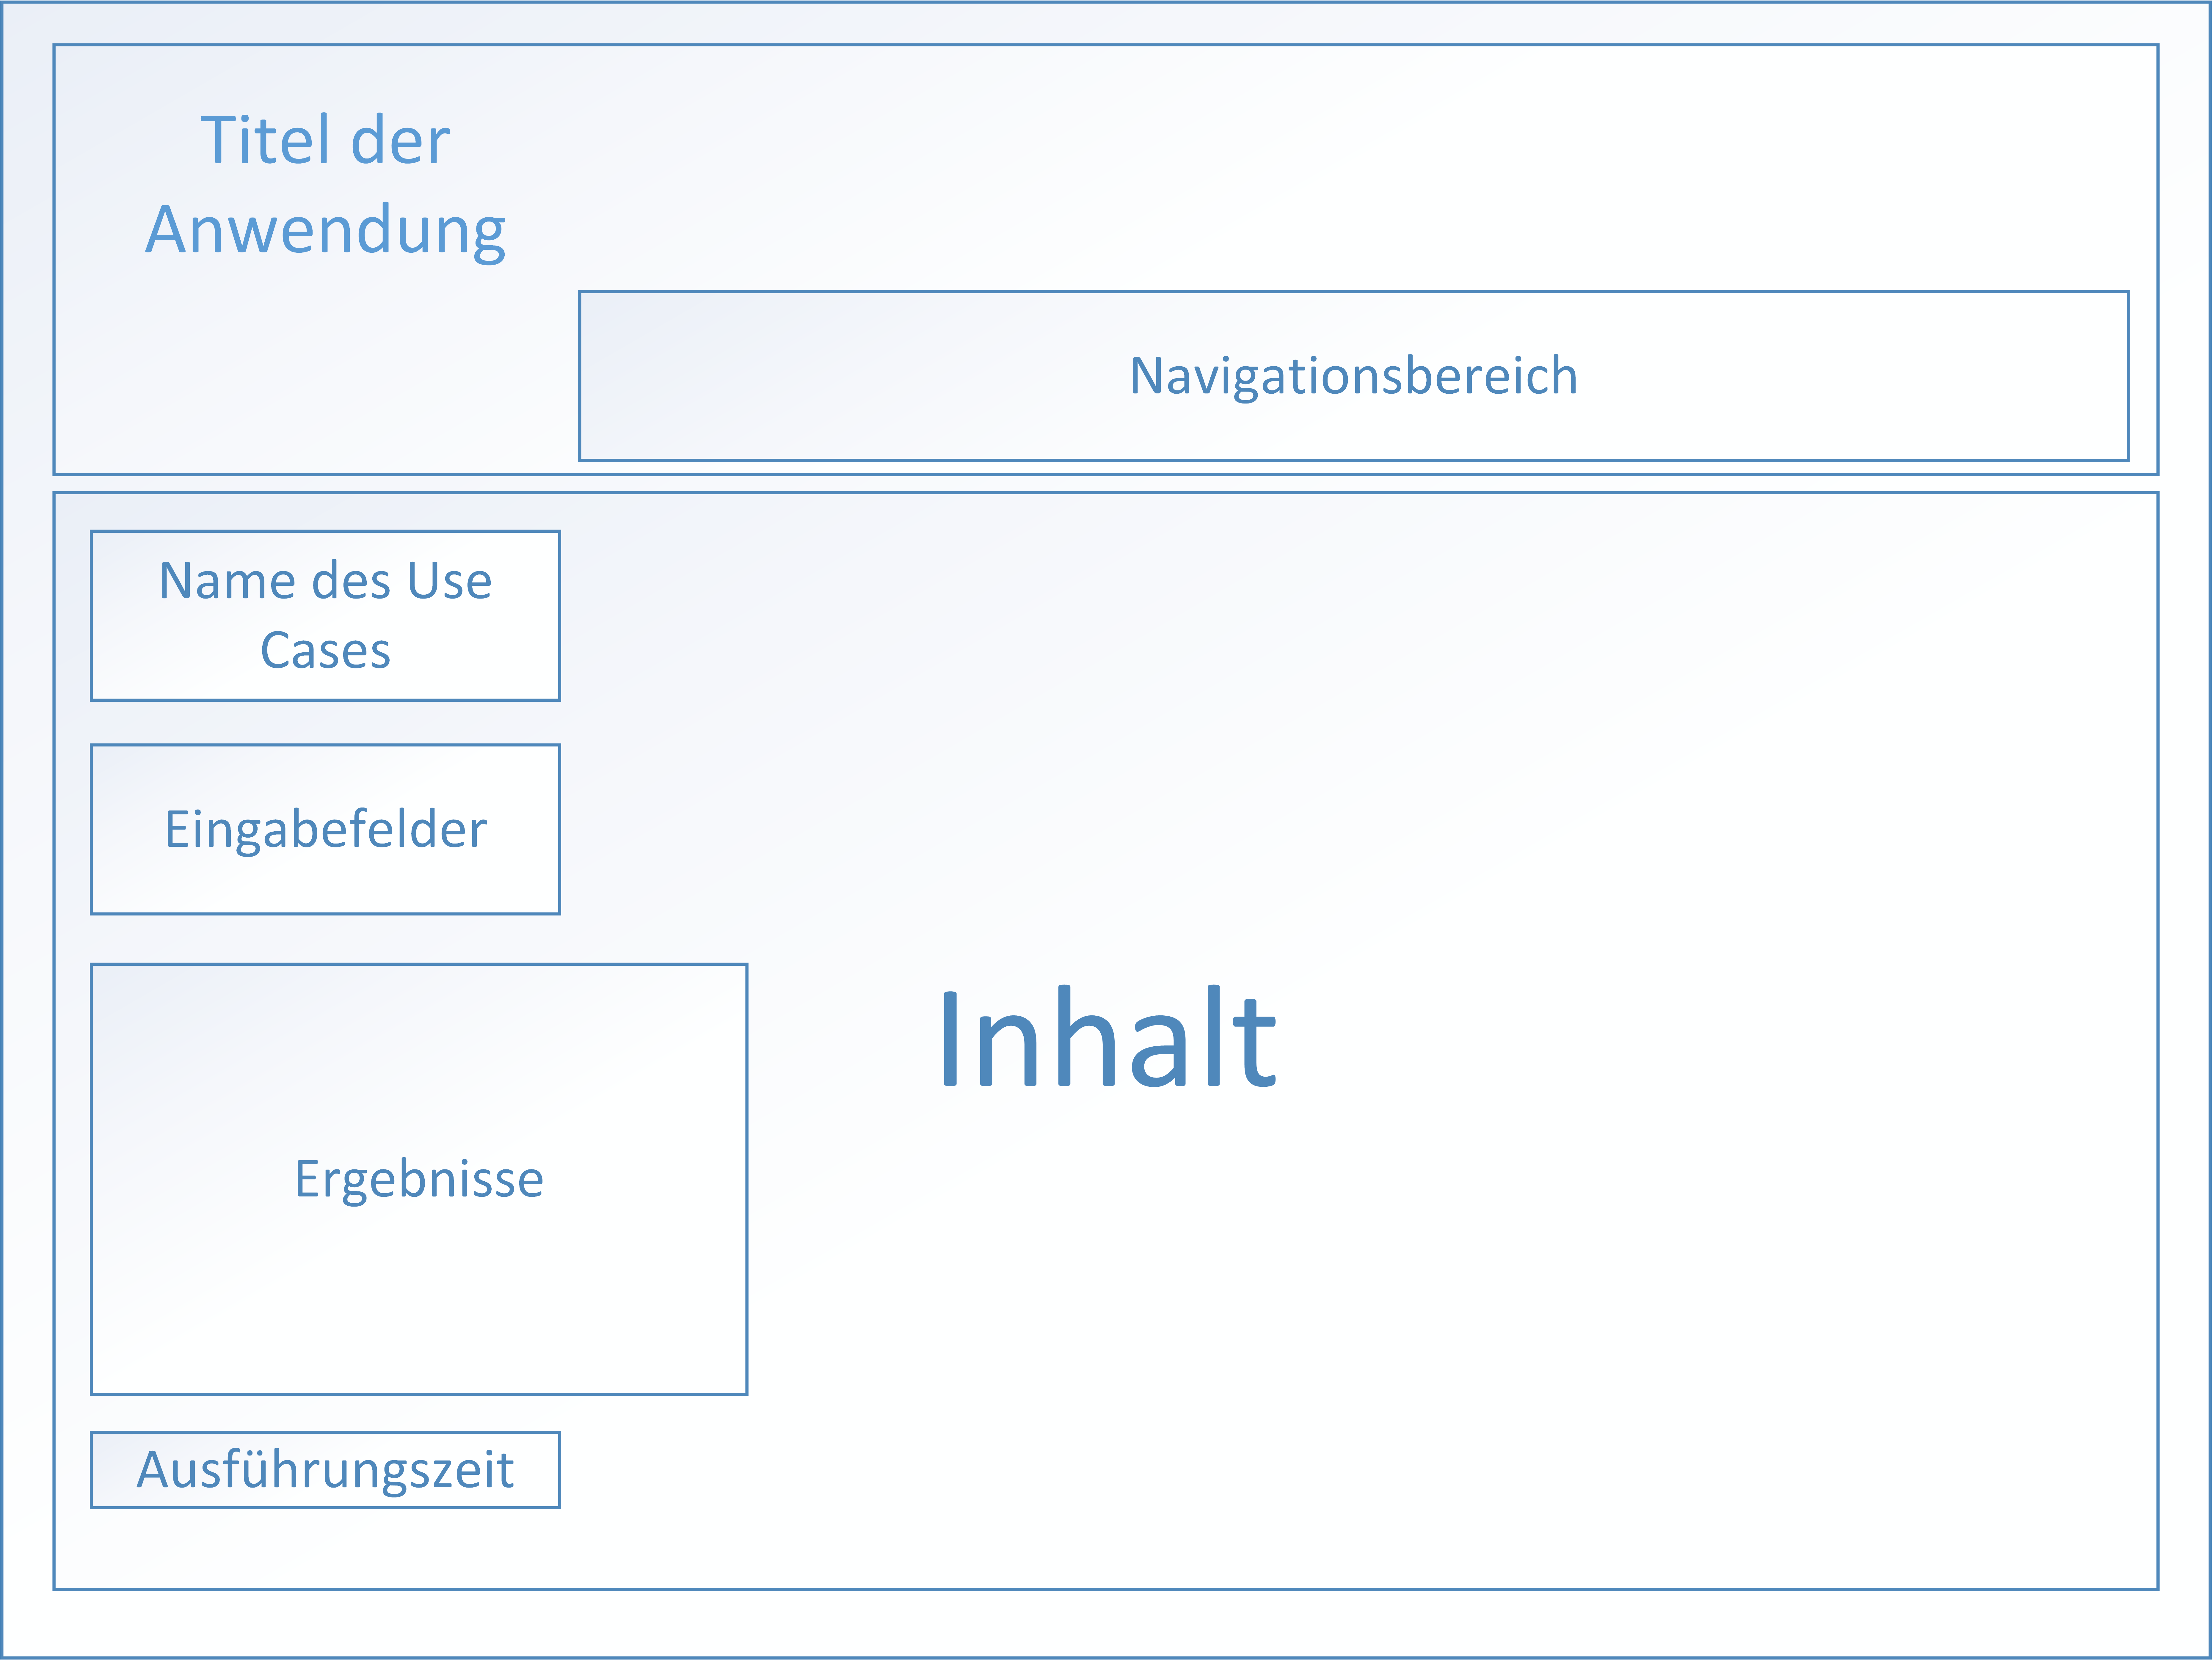
\includegraphics[scale=0.6]{images/01_oberflaechengestaltung.png}
    \caption{Schematische Darstellung der Weboberfläche}\label{fig:oberflaeche}
\end{figure}

Dabei wurde darauf geachtet, dass sich der Navigationsbereich dynamisch generiert, sodass dieser nicht jedes mal neu erstellt werden muss wenn ein neuer Use Case hinzu kommt. Der Inhaltsbereich, welcher Ein- und Ausgabemaske darstellt wird abhängig von der Eingabe im Navigationsbereich geladen. 

\subsubsection{Implementierungskonzept}
Bei der Implementierung wurde sich für das Vaadin-Framework entschieden, da es die schnelle Erstellung einer Webseite mittels Java ermöglicht. Dabei müssen keine HTML- oder JavaScript-Dateien bearbeitet werden. Die Elemente und das Layout werden mit Hilfe von Vaadin-Objekten direkt im Quellcode erzeugt. Die Kommunikation zwischen Webseite und Anwendungsserver wird vollständig durch das Vaadin-Framework gekapselt. Abbildung \ref{fig:datenfluss} modelliert den Datenfluss der gesamten Anwendung. Hier ist der Datenfluss zwischen Ein- und Ausgabemaske der Anwendung im Browser und der Datenbank besonders relevant. Allerdings kapseln sowohl das Vaadin-Framework als auch die Treiber der MongoDB den größten Teil hiervon. Es kann nur Einfluss auf die Datenverarbeitung im Quellcode auf dem Anwendungsserver genommen werden. Dieser bekommt vom GUI verkörpert durch die Vaadin-Objekte die Eingabewerte in Form von einfachen Java-Datentypen wie String oder Integer (In der Abbildung als ,,Object`` dargestellt). Die MongoDB erwartet als Eingabe ein Objekt vom Typ DBObject. Aus mehreren ineinander verschachtelten DBObjects wird der Query zusammengestellt. Der Rückgabewert der MongoDB besteht entweder aus einem DBObject, oder einem AggregationOutput, welcher eine Liste von DBObjects verkörpert (In der Abbildung als ,,Object*`` dargestellt). 

\begin{figure}[H]
    \centering
    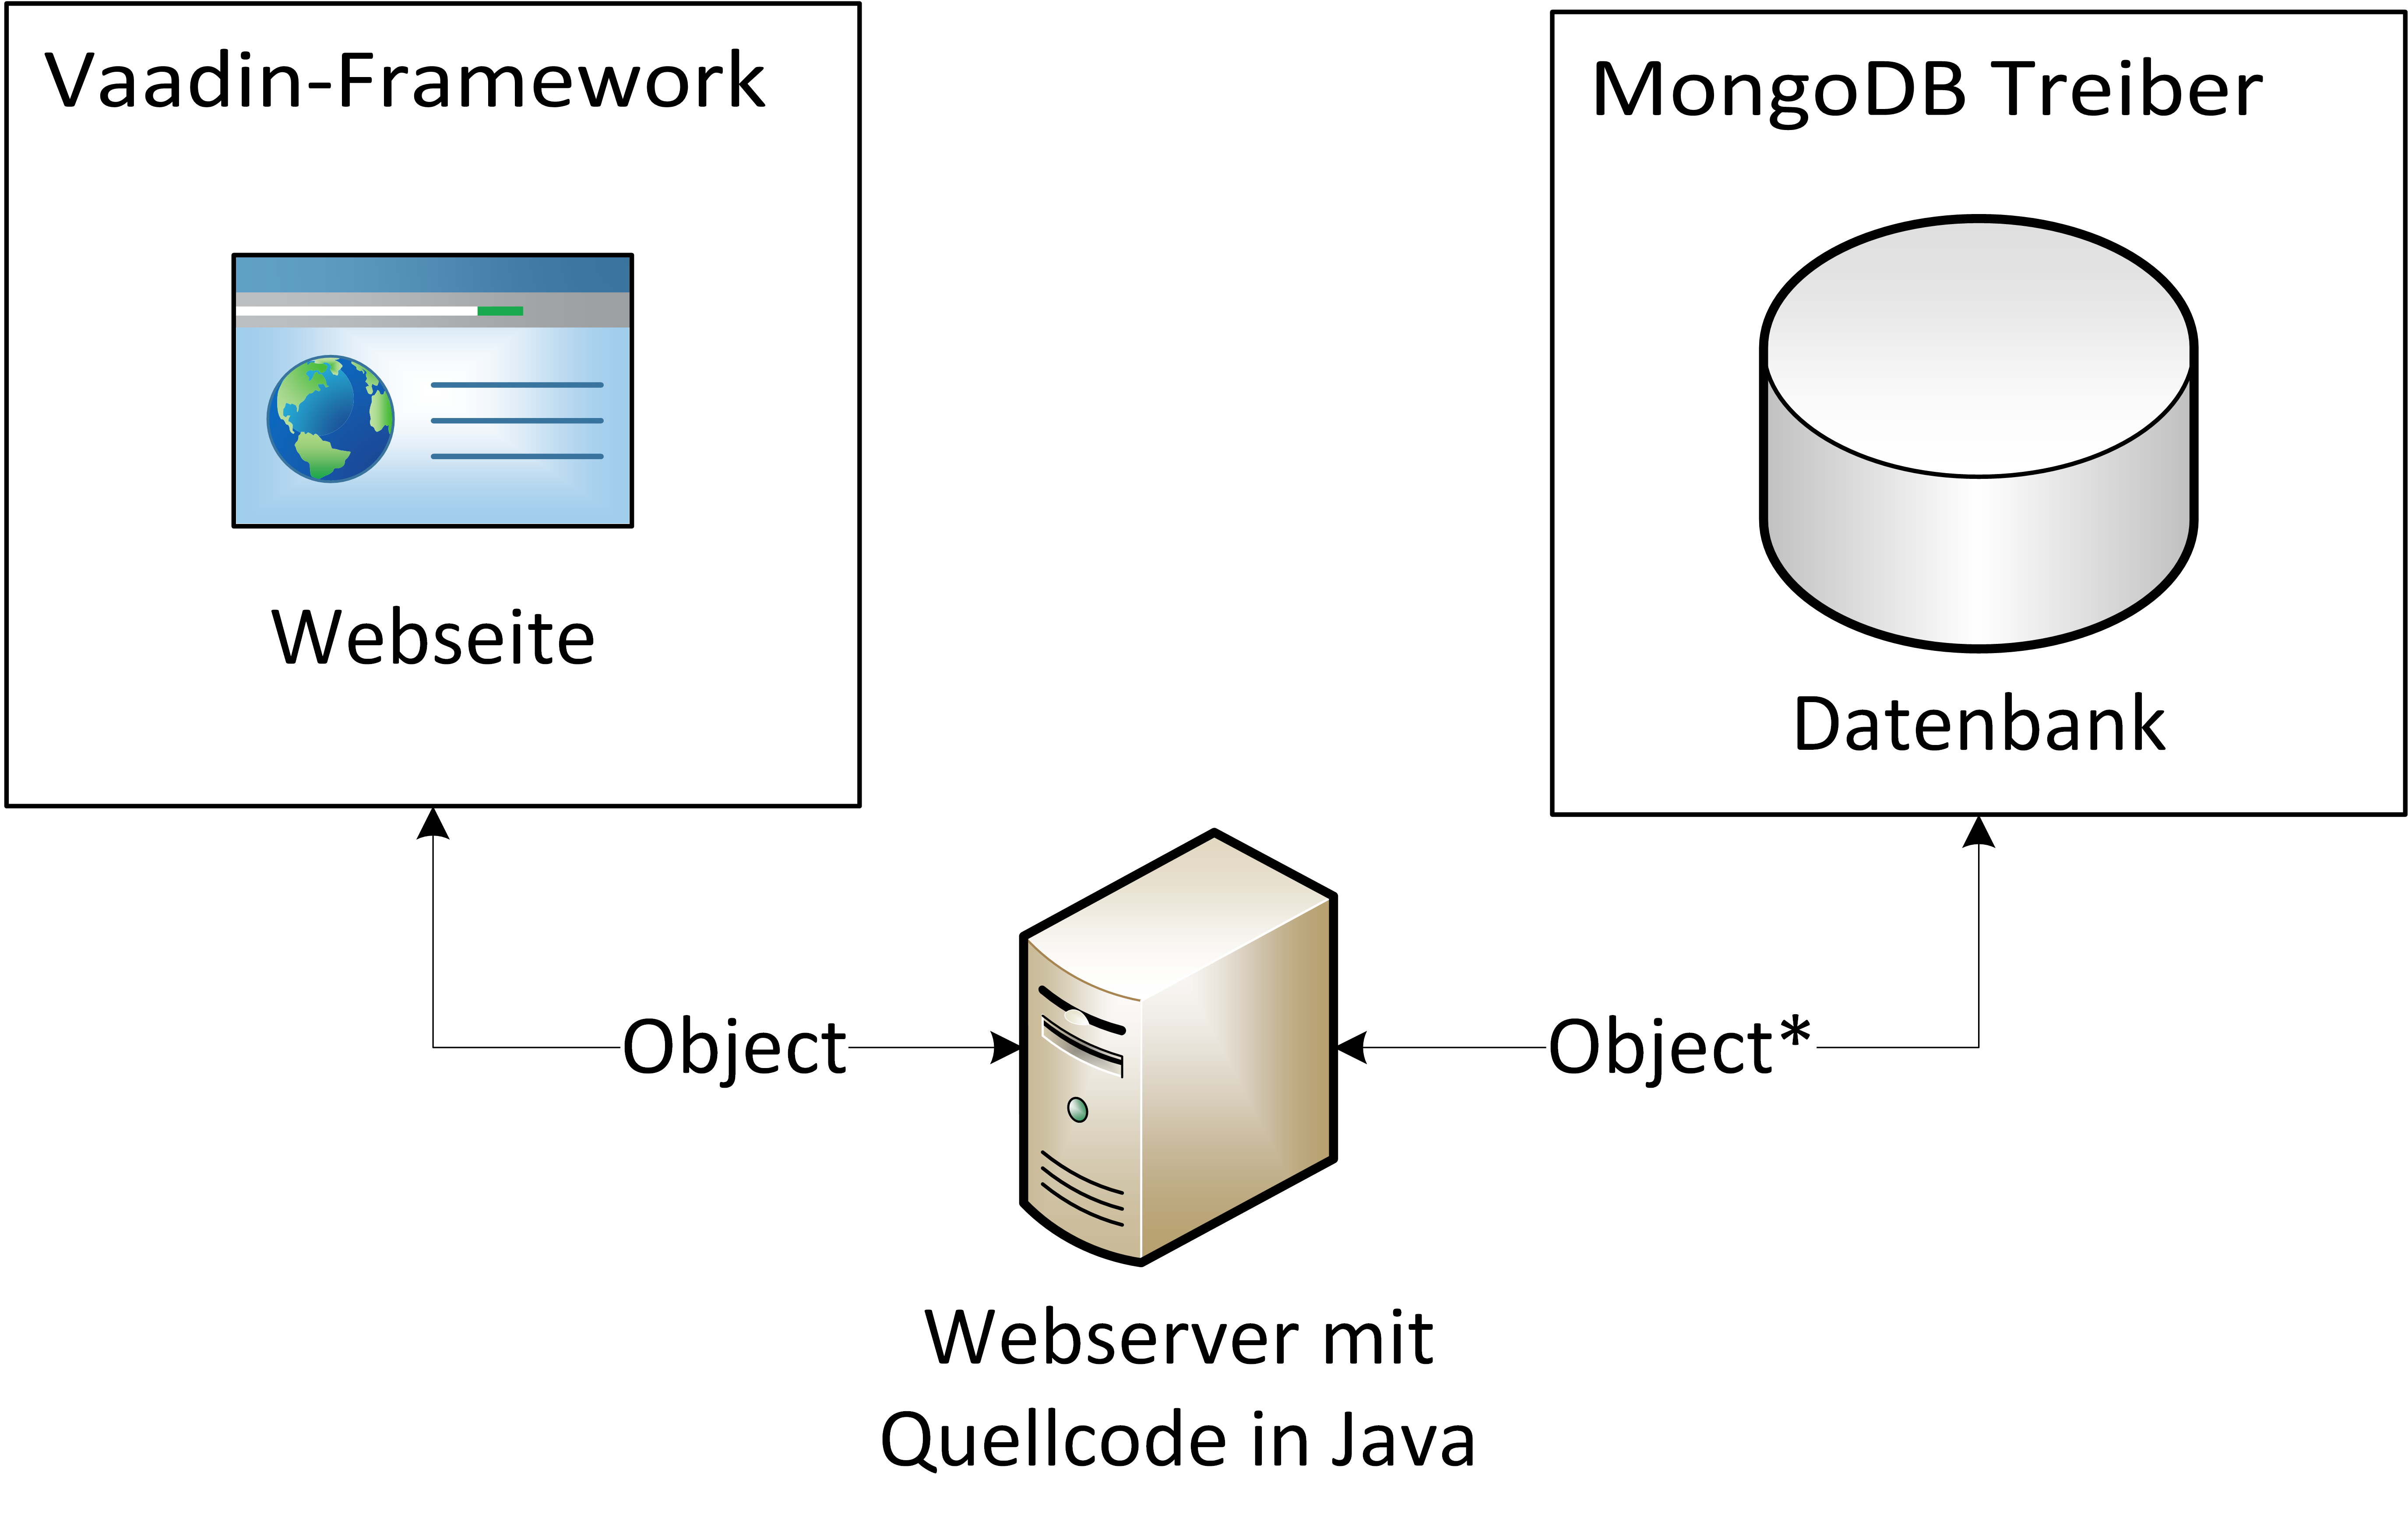
\includegraphics[scale=0.6]{images/01_datenfluss.png}
    \caption{Exemplarischer Datenfluss zwischen Anwendung und Datenbank}\label{fig:datenfluss}
\end{figure}

\subsubsection{Schnittstelle der Anwendung zur Datenbank} \label{dbdriver}

die Implementierung programmiertechnisch unterschiedliche Anfragen vorstellen.
Eine Reihe ähnlich gearteter Selects ist da sicher nicht so hilfreich.


Die vorgestellte Java-Anwendung nutzt den von MongoDB bereitgestellten Java Treiber um eine Kommunikation mit der Datenbank herzustellen. Hierbei wird über den Treiber eine Verbindung zum Server hergestellt, auf dem der anzusteuernde Query-Server installiert ist. Auf diesem werden über einfache Funktionsaufrufe die Datenbank und die Collection selektiert. 

Ein Query wird, wie bereits erwähnt, durch verschachtelte DBObjects dargestellt. Ein DBObject verlangt im Konstruktor einen Key und einen Value. Als Value kann wiederum ein DBObject eingesetzt werden. Dies wird in Use Case fünf, vergleiche Anhang \ref{use_cases}, besonders deutlich, wo der \textit{nequery} in den \textit{query} eingesetzt wird. Use Cases sechs und acht stellen dagegen wesentlich komplexere Verschachtelungen dar. 
Anschließend wird der fertige Query auf dem Objekt der Collection ausgeführt. Hierfür bietet diese alle Methoden an, die auf der Konsole auf der Collection auch ausgeführt werden können, wie beispielsweise find(), count() und distinct(). Der Rückgabewert hier ist eine Liste von DBObjects wenn das Ergebnis ein Dokument verkörpert oder AggregationOutput wenn es sich um mehrere Dokumente handelt.

Der Vergleich der beiden Queries, wie sie auf der Konsole und im Quellcode konstruiert wurden, zeigt deutlich dass ein DBObject eine BSON-Zuweisung von Key zu Value \textit{\{ ’’Key’’ : ’’Value’’ \}} verkörpert.

\subsubsection{Test der Anwendng}
Die acht vorgestellten Use-Cases haben sich vollständig mit Hilfe von MongoDB abbilden lassen. In Tabelle \ref{tab:ausfuehrungszeiten} wird aufgezeigt, wie viel Zeit benötigt wurde um die einzelnen Anfragen zu bearbeiten. Hierbei ist jedoch relevant zu erwähnen, dass die Geschwindigkeit der Beantwortung von der Auslastung der Server abhängig ist, die in diesem Fall nicht konstant war. Auffällig ist, dass in einigen Fällen die Anwendung eine schnellere Antwortzeit hatte, als eine Abfrage direkt auf dem Server. Dies verdeutlicht, dass MongoDB ein großes Potenzial in der Performance hat.

\begin{table*}[h]
\caption{Ausführungszeiten der Use Cases in Sekunden}
\centering
\begin{tabular}{|p{3cm}|p{4cm}|p{4cm}|}
\hline
     & Robomongo (in sec) & Anwendung (in sec) \\
\hline
Use Case 1 & 0,339 & 0,126 \\
\hline
Use Case 2 & 0,534 & 0,137 \\
\hline
Use Case 3 & 0,447 & 0,124 \\
\hline
Use Case 4 & 0,319 & 0,577 \\
\hline
Use Case 5 & 0,111 & 0,161 \\
\hline
Use Case 6 & 0,517 & 0,461 \\
\hline
Use Case 7 & 0,173 & 0,125 \\
\hline
Use Case 8 & 0,078 & 0,039 \\
\hline
\end{tabular}
\label{tab:ausfuehrungszeiten}
\end{table*}


Die für die Anfragen benutzten Eingaben in den Tests lauten wie folgt: 

\begin{itemize}
\item [UC1:] \textit{’’Datenbank’’}
\item [UC3:] \textit{’’Prof. Harm Knolle’’}
\item [UC4:] \textit{’’SS 07’’}
\item [UC7:] \textit{’’Datenbank’’}
\item [UC8:] \textit{’’Datenbank’’}
\end{itemize}

Durch Indizierung von Attributen kann die Ausführungszeit von Queries um den Faktor zehn verbessert werden. Dies wurde während der Tests empirisch bewiesen. In den gegebenen Use-Cases sind vor allem der Erstprüfer, das Thema der Arbeit, das Zeugnis und die Firma Attribute, die von größerer Relevanz sind. Daher bietet es sich an diese Attribute zu indizieren, um die Performance der Queries zu erhöhen. Die in Tabelle \ref{tab:ausfuehrungszeiten} aufgelisteten Zeiten wurden bereits durch Indizierung generiert. Folgende Befehle wurden für die Erstellung der Indizes ausgeführt:

\begin{lstlisting}[caption={Befehle zur Erstellung der Indizierung},language=java,captionpos=t,numbers=none,basicstyle=\scriptsize,numberstyle=\tiny,breaklines=true]
db.abDBsimpleCSV.createIndex({Thema der Arbeit":1},{name:"thema"})
db.abDBsimpleCSV.createIndex({"1. Pruefer":1},{name:"pruefer"})
db.abDBsimpleCSV.createIndex({"Zeugnis":1},{name:"abschluss"})
db.abDBsimpleCSV.createIndex({"Firma":1},{name:"unternehmen"})
\end{lstlisting}\label{lst:query1}
